%====================================================
%
% Author: DR. XAVIER NOUMBISSI NOUNDOU
%
%====================================================
\documentclass[12pt, a4paper]{article}
\NeedsTeXFormat{LaTeX2e}

%---------------------------- PACKAGE INCLUSION -------------------------------
% This group renders characters clearer and more precise

\RequirePackage[bitstream-charter,cal,expert]{mathdesign}
\RequirePackage{latexsym}

\usepackage{geometry}
\geometry{a4paper,
		  %showframe=true,
		  %margin=2.75em,
		  %a4paper,
		  %total={170mm,257mm},
		  top=3.5em,
		  left=3em,
		  right=3em,
		  bottom=3.39em
		  }

\usepackage[default]{cantarell}
\usepackage{graphicx}
\usepackage{xspace}
\usepackage[parfill]{parskip} % Activate to begin paragraphs with an empty line rather than an indent
\usepackage{paralist} % very flexible & customisable lists (eg. enumerate/itemize, etc.)
\usepackage{listings} % for lstset definitions
\usepackage{url}
\usepackage{subfig} % make it possible to include more than one captioned figure/table in a single float
\usepackage{epsfig}
\usepackage{booktabs}
%\usepackage{enumitem} %funny itemize icons
\usepackage{verbatim}
\usepackage{tcolorbox}

\usepackage{footnote}
\makesavenoteenv{tabular}
\makesavenoteenv{table}

\usepackage{pagecolor}

\usepackage{amsmath}
\newcommand{\mathbold}[1]{\text{\textbf{#1}}}

\usepackage{xcolor}
\definecolor{yerothColorOrange}{RGB}{242, 161, 0}   
\definecolor{yerothColorBlue}{RGB}{77, 93 , 254}
\definecolor{yerothColorRed}{RGB}{254, 48 , 48}
\definecolor{yerothColorGray}{RGB}{198, 198, 198}
\definecolor{yerothColorDarkgray}{RGB}{60, 60 , 60}
\definecolor{yerothColorIndigo}{RGB}{83, 0, 125}
\definecolor{yerothColorGreen}{RGB}{2, 160, 70}
\definecolor{forestgreen}{RGB}{2,160,70}    
\definecolor{mediumblue}{RGB}{7,43,205}    
\definecolor{firebrickred}{RGB}{178,34,34}
\definecolor{listingray}{gray}{0.9}
\definecolor{lbcolor}{rgb}{0.9,0.9,0.9}
\definecolor{darkgreen}{rgb}{0,0.35,0}
\definecolor{medgreen}{rgb}{0,0.5,0}
\definecolor{lightgreen}{rgb}{0.5,0.7,0.5}
\definecolor{pmcolour}{rgb}{0.5,0.7,0.5}
\definecolor{medgrey}{rgb}{0.6,0.6,0.6}
\definecolor{purplish}{rgb}{0.4,0,0.6}
\definecolor{brightred}{rgb}{1,0.2,0.2}

\newcommand{\diplinfn}{DR.\xspace}

\newcommand{\yerothrd}{\textcolor{yerothColorGreen}
			{\textsc{\textcolor{yerothColorRed}{YEROTH}}$_{\text{r\&d}}$\xspace}}


\newcommand{\yerotherpblack}{YEROTH--ERP--$3.0$\xspace}

\newcommand{\yerotherp}{\textcolor{yerothColorBlue}{\sc YEROTH--ERP--$3.0$}\xspace}

\newcommand{\myfullacademicname}{DR. XAVIER NOUMBISSI NOUNDOU\xspace}

\usepackage{hyperref}
\hypersetup{
    colorlinks,
	pagebackref,
    citecolor=medgreen,
    linkcolor=purplish,
    breaklinks,
    pdftex,
    bookmarks,
    plainpages=false,
	pdftitle={\yerotherpblack software--system inventory stock recommended hardware
				authored by: ''\myfullacademicname''},
    pdfauthor={\myfullacademicname}
}

%--------------------------------------------------------------------------------

%---------------------------- COMMANDS DEFINITION -------------------------------
\newcommand{\diplinf}{\emph{DR.}\xspace}
\newcommand{\mycheckmark}[1]{\textcolor{#1}{$\checkmark$}\xspace}

\newcommand{\myenumitem}[1]{\emph{#1}\xspace}
\newcommand{\yerenalert}{\emph{yeren-alert}\xspace}

\newcommand{\pos}{point--of--sale~software--system\xspace}

\newcommand{\mysql}{MySQL\xspace}
\newcommand{\mysqlcolored}{\textcolor{yerothColorBlue}{My}\textcolor{yerothColorOrange}{SQL}\xspace}

\newcommand{\featuresummary}[2]{\textbf{\textcolor{#1}{\textsc{#2}}}}

\newcommand{\chapintro}[1]{\textcolor{purplish}{\emph{#1}}\xspace}

\newcommand{\moneybold}[1]{$\mathbf{#1}\ \euro{}$\xspace}

\newcommand{\money}[1]{$#1\ \euro{}$\xspace}

%--------------------------------------------------------------------------------

\usepackage[T1]{fontenc}
\newcommand{\changefont}[3]{
\fontfamily{#1} \fontseries{#2} \fontshape{#3} \selectfont}
\changefont{cmss}{m}{n}

\renewcommand\labelenumi{\theenumi)}

\pagenumbering{gobble}

\usepackage{fancyhdr}
\pagestyle{fancy}
\renewcommand{\headrulewidth}{0pt}
\rhead{}
\lhead{}
\lfoot{{\small Author: \myfullacademicname}}
\rfoot{{\small Version of --~\today~--}}
\cfoot{}

\clubpenalty = 10000
\widowpenalty = 10000
\displaywidowpenalty = 10000

\usepackage{sectsty}

\sectionfont{\fontsize{15}{18}\selectfont}


\begin{document}

{\bf \Large \yerothrd} {| \sc \scriptsize \yerotherpblack point--of--sale recommended hardware}

\vspace{2.5em}


\parbox{27em}{\LARGE \yerotherpblack Point--Of--Sale Recommended Hardware}

\vspace{0.5em}

\section{Barcode Scanner}
\vspace{-3.7em}

\begin{table}[!htbp]
\begin{tabular}{lr}
\parbox{25em}{
We recommend, but not exclusively, the use 
of barcode scanner:
\textbf{''~Xfox FJ--5 USB Plug and Play Automatic
Barcode Scanner~''} (approx.~\money{17}).
\vspace{-3em}
}

&

\parbox{17em}{
\begin{center}
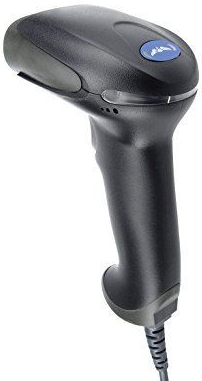
\includegraphics[scale=0.2]{images/xfox-fj-5-usb-plug-and-play-automatic-barcode-scanner.png}
\caption*{Barcode Scanner}
\end{center}
}
\end{tabular}
\end{table}

\vspace{-0.8em}
\section{Thermal Printer}
\vspace{-2.7em}

\begin{table}[!htbp]
\begin{tabular}{lr}
\parbox{25em}{
We recommend, but not exclusively,
the use of thermal printer: 
\textbf{''~Epson~TM-T20ii~Point~of~Sale~Thermal~Printer~''}
(approx.~\money{100}).
\vspace{-3em}
}

&

\parbox{17em}{
\begin{center}
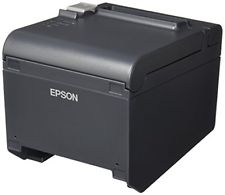
\includegraphics[scale=0.27]{images/epson-tm-t20-pos-thermal-printer.png}
\caption*{Thermal Printer}
\end{center}
}
\end{tabular}
\end{table}

\vspace{0em}
\section{Cash Drawer}
\vspace{-3.1em}

\begin{table}[!htbp]
\begin{tabular}{lr}
\parbox{25em}{
We recommend, but not exclusively,
the use of cash drawer:
\textbf{''~HP~QT457AT~''} (approx.~\money{90}).
\vspace{-3em}
}

&

\parbox{17em}{
\begin{center}
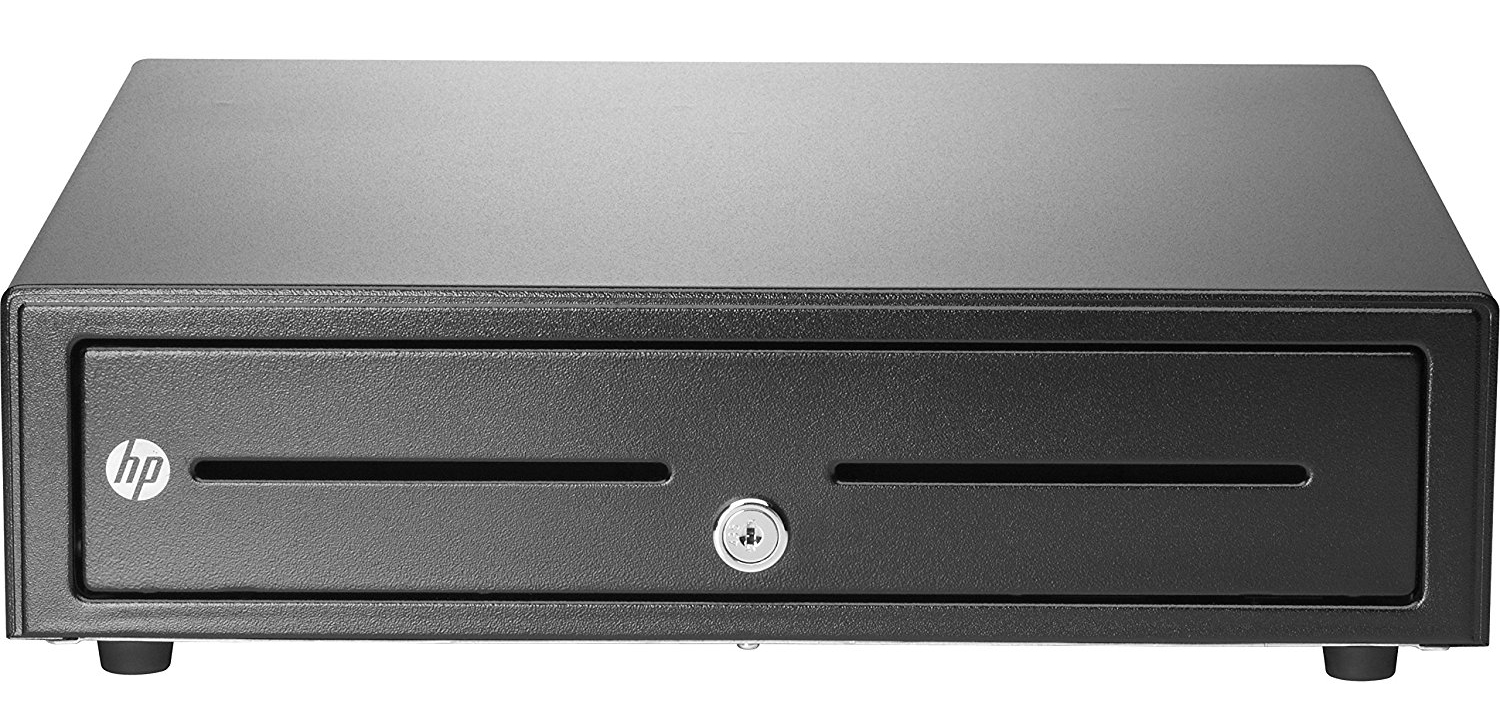
\includegraphics[scale=0.07]{images/hp-cash-drawer.png}
\caption*{Cash Drawer}
\end{center}
}
\end{tabular}
\end{table}

\vspace{-0.5em}
\section{Touch Screen Monitor}
\vspace{-3.8em}

\begin{table}[!htbp]
\begin{tabular}{lr}
\parbox{25em}{
We recommend, but not exclusively,
the use of touch screen
monitor: \textbf{''~ASUS~15.6"~LCD~Monitor~(VT168H)~''} (approx.~\money{155}).
\vspace{-3em}
}

&

\parbox{17em}{
\begin{center}
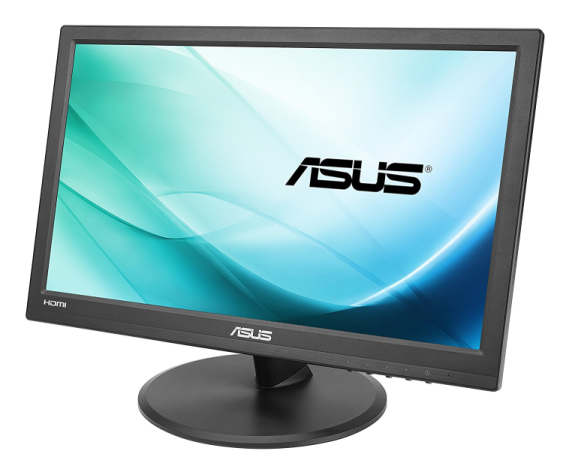
\includegraphics[scale=0.14]{images/asus-15_6-lcd-monitor.png}
\caption*{Touchscreen Monitor}
\end{center}
}
\end{tabular}
\end{table}

\vspace{-1em}
\section{Computer}
\vspace{-3.71em}

\begin{table}[!htbp]
\begin{tabular}{lr}
\parbox{25em}{
We recommend, but not exclusively, the use
of desktop computer:
\textbf{''~Lenovo~Thinkcentre~M$\mathbf{720}$~Small~Form~Factor~(SFF)~''}
(approx.~\money{450}).
\vspace{-3em}
}

&

\parbox{17em}{
\begin{center}
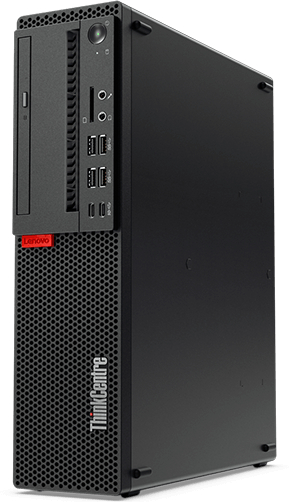
\includegraphics[scale=0.14]{images/lenovo-thinkcentre-m710sff-hardware.png}
\caption*{Computer}
\end{center}
}
\end{tabular}
\end{table}
	
\end{document}

